\PassOptionsToPackage{unicode}{hyperref}
\PassOptionsToPackage{hyphens}{url}
%

\documentclass[12pt, a4paper]{article}
\usepackage[a4paper,margin=1in]{geometry}
\setlength\parindent{0pt}
\usepackage{mathptmx}
\usepackage{amsmath,amssymb}
\usepackage[T1]{fontenc}
\usepackage[utf8]{inputenc}
\usepackage{textcomp}
\usepackage{pgfplots}
\usepackage{verbatim}
\usepackage{hyperref}
\usepackage{graphicx}
\graphicspath{{img-tables/}}

\author{Mattia Buzzoni, Artificial Intelligence Master Degree, ID number 0001145667
\\Leonardo Mannini, Artificial Intelligence Master Degree, ID number 0001135209
\\Mirko Mornelli, Artificial Intelligence Master Degree, ID number 0001113084
\\Riccardo Romeo, Artificial Intelligence Master Degree, ID number 0001145681
\\Diego Rossi, Artificial Intelligence Master Degree, ID number 0001138652}
\date{05-23-2025}
\title{A Song of Ice and Fire}

\begin{document}
\maketitle

\section{Introduction}
\label{introduction}
The analysis of narrative structures is a wide field that shows the complexity of human society and imagination. A specific area, narrative fiction, especially epic fantasy, is a good source for analyzing structures and characters. The series A Song of Ice and Fire by George R. R. Martin is a very complex example of modern fantasy. Its large number of characters, changing alliances, and complex plots make it an interesting topic for both literary and computational study.
This project is part of digital literary studies, combining narrative analysis and network science. We focus on the social structures in A Song of Ice and Fire, looking at character interactions in the five published books. These books describe a growing universe with hundreds of characters, each playing a part in a large political and personal story.

To understand the structure of these character interactions, we use Social Network Analysis (SNA). SNA lets us represent the story as a graph, where characters are nodes and their interactions are edges. By studying these networks with computational tools, we want to get quantitative information about the story's structure. Specifically, we look at how character importance, community structures, and connections change across the five books.

With this combined approach, our project aims to explore the rich world of these books from a new analytical viewpoint. We also want to show that using network-based methods is a valid way to study complex literary works.

\section{Problem and Motivation}
\label{problem-and-motivation}

This project investigates the underlying structure of character interactions within the fantasy saga \textit{A Song of Ice and Fire}, focusing on the first five books of the series. The central aim is to explore how characters are positioned within the social landscape of the narrative and to assess their importance across different stages of the story. Unlike many traditional narratives with a single protagonist, this saga features a complex and distributed set of characters whose relevance varies considerably over time and context.

The problem we seek to address is the difficulty of identifying and evaluating character centrality in such a fragmented and multi-perspective storyline. In a literary universe composed of hundreds of characters, each with their own alliances, roles, and trajectories, determining who the key figures are and how these figures influence or connect with others, presents both a narrative and analytical challenge. This is particularly important in a work like \textit{A Song of Ice and Fire}, where shifts in power, betrayal, and character deaths play a crucial role in the progression of the plot.

The motivation for this work lies in the potential of structural analysis to offer a deeper and more systematic understanding of narrative dynamics. By investigating which characters act as central nodes, which form cohesive groups, and how the overall structure evolves from one book to the next, we aim to provide insights that complement traditional literary interpretation. This approach enables a more objective reflection on character importance, the density of relationships, and the organization of fictional societies.

The main contribution of the project is to map and analyze the evolving network of character interactions across the five books, highlighting patterns of centrality, influence, and group formation. Through this, we hope to shed light on the complex mechanisms of storytelling in epic fantasy and to demonstrate how structural perspectives can enrich our understanding of literary worlds.
\section{Datasets}
\label{datasets}

The character network for Game of Thrones (the A Song of Ice and Fire novels) comes from a dataset available to the public. 
This dataset creates connections (edges) between characters based on when their names appear close to each other in the text. 

Specifically, an edge is made if two characters' names are within 15 words of each other in the books. 
This method, called co-occurrence, was made popular by Beveridge and Shan's Network of Thrones study. 
It's often used as a good way to guess if characters are in the same scene, talk to each other, or are mentioned together. 

The 15-word window is meant to be small enough to show a direct connection but large enough to catch most immediate interactions. Any window size can seem a bit random and might not perfectly catch every detail of interactions (for example, quick mentions could be missed, or names that are not related but appear in a crowded part of the text might be linked). However, it gives a consistent way to define interactions from the text that others can repeat. Basically, a link in the network means there's a contextual relationship. This could mean that two characters talked to each other, talked about each other, or were mentioned together. The strength of a connection (its weight) is the number of times these co-occurrences (interactions) happen between two characters. 

The dataset has CSV files (one for each book) that list pairs of character names and how many times they co-occur. Using this data, we built an undirected, weighted graph for each of the five books, and also a combined network for all books. Each character is a node, and an edge between two nodes means those characters were mentioned near each other in the text. The weight on each edge shows how many times the characters appear together. This acts as a measure of how strong their relationship is in the story (for example, characters who meet or talk often will likely have a higher weight).


\subsection*{Data Collection and Pre-processing}

The character-co-occurrence edge lists we analyse come from a community dataset on Kaggle entitled Game of Thrones Network.
The dataset's author parsed the full text of the five published novels and recorded every pair of character names that occur within a 15-word sliding window.

In our own notebook, we performed only light additional cleaning. 
The combined graph has 796 nodes and 2 823 weighted edges.

\subsection*{Tools Used}
We used Python and its libraries for all data processing and analysis. Specifically, we used pandas for handling data and NetworkX for creating graphs and doing network analysis. We used other packages like Matplotlib for plotting.  All our code and processed data are available in a public GitHub repository.
\section{Validity and Reliability}

\label{validity-and-reliability}
Because the dataset came from a user on Kaggle and not from official text notes, the data might not be perfectly accurate. Possible problems include missed co-occurrences, wrong edges, or names that are not consistent. Even with these issues, the dataset seems to be quite valid because its patterns match the known story of the books well. In fact, one of our goals was to check the dataset by seeing if known story structures appeared in the network analysis. 

More than just qualitative checks, the dataset's reliability is supported by the fact that it can be reproduced and is consistent with other studies. This means anyone could create the co-occurrence network again from the original text and would 
likely get a very similar list of connections. 


For internal consistency, we made sure to do the analysis the same way for each book, we used the same metrics and algorithms 
 for all five networks, with the same settings, so comparisons between books should be valid. In short, even if the dataset isn't perfect, 
 the evidence shows it's accurate enough for a useful analysis: the network patterns that appear seem to reflect the Game of Thrones story, 
 and the method can be repeated. 
 
 These results show a clear consistency with the "A Song Of Ice And Fire" story, which makes us more confident that the dataset is valid and also reliable.
 
 

\section{Measures and Results}
\label{measures}
To measure the roles and importance of characters in the network, we calculated several centrality measures and other graph metrics. Each of these measures shows a different side of a character's importance or position in the social network. Below, we will briefly explain each metric and then talk about what we found for each book and for the whole series.

\subsection*{Degree Centrality}
Degree centrality, 
is the number of edges each node has. 
A high degree means the character interacts with or is
 mentioned with many others, making them a center of the network. 
 For instance, if a character is in scenes with 10 different characters,
  their degree centrality is 10. 
  This measure naturally shows a character's
   visibility and direct involvement in the story. 
   In our study, Tyrion Lannister has the highest 
   degree centrality in all five books. 
     Tyrion's job as a counselor and his travels bring him into 
     contact with many different characters.
      Degree centrality gives a basic ranking of characters 
      by how connected they are, but it doesn't look at who 
      they are connected to.

\subsection*{Eigenvector Centrality}
Eigenvector centrality is a more advanced measure of influence.
 It looks at the quality of connections, not just the number, 
 giving higher scores to nodes connected to other highly connected nodes.
  This measure can show 
   characters who are at the center of the main network groups. 
   Our results for eigenvector centrality were very simila
    to the degree centrality rankings for the top characters 
    – main characters like Tyrion, Jon Snow, Daenerys Targaryen,
     and Cersei Lannister scored high. This suggests that 
     these characters not only have many connections but are also
      connecting to each other or to other key people, forming a 
      close-knit core of important characters. On the other hand,
       a character like Daenerys is an interesting example: in 
       the early books, her degree might be fairly high.

\subsection*{Katz Centrality}
Katz centrality is an extension of eigenvector centrality:
 every character starts with a small baseline score and then
  gains additional influence from walks of length two, three, 
  and so on, each step counting a little less than the previous one. 
  

When we compute the measure on the full five-book network, 
Tyrion Lannister emerges as the first one,
 with Jon Snow in a close second place. 
 Immediately behind them come Jaime Lannister, 
 Cersei Lannister, and Stannis Baratheon. Jon's score climbs book 
 after book, reflecting how his storyline gradually connects the 
 Night's Watch, the wildlings, the northern houses, and even the 
 Iron Throne via correspondence. 

This metric  reinforces what simpler measures already indicated, 
Tyrion and Jon dominate the narrative, but it adds something. 
It shows Jon's influence catching up over time and highlights 
characters such as Stannis and Arya, who do not have the 
highest degree counts yet serve as effective conduits that
 link otherwise distant parts of the network.


\subsection*{Closeness Centrality}
Closeness centrality measures how close a character is to all 
other characters in the network, based on graph distance. 
Officially, it's the inverse of the average shortest path length 
from one node to all other nodes. A character with high closeness 
centrality can reach every other character through just a few steps 
on average. 
We found that characters like Tyrion and 
 Cersei Lannister often had some of the shortest average 
 distances to others. Tyrion interacts with 
 many groups. Cersei is in a central place in King's Landing 
 and interacts with various people, so she's never far from any storyline. 
 Interestingly, Petyr Baelish also had a 
 fairly high closeness centrality in the early books even if it is a secondary character,
  making him an almost universal 
 connector in the network. So, closeness centrality 
 highlighted characters who act as hubs connecting 
 communities.

\subsection*{Betweenness Centrality}
Betweenness centrality measures how often a node is on the 
shortest path between any two other nodes. It effectively 
finds the ``bridge'' characters in the network, those who 
connect different communities or whose presence is key for 
information to flow in the network. A character with high 
betweenness centrality might not have the most connections, 
but they are at important points between storylines. 
Our betweenness analysis gave some of the most interesting 
results, as it pointed out a few characters we didn't expect. 
For example, Stannis Baratheon had the highest betweenness 
centrality in the combined five-book network. This result 
seems surprising at first because Stannis is a major character but 
fairly isolated (he doesn't interact with many other main characters 
besides his own followers). However, the network structure explains 
it: Stannis and his group form a bridge between the King's Landing 
storyline and the Wall (and later the northern conflict). 
If you ``remove'' Stannis and his connecting nodes, 
the network splits – his followers 
and their interactions with other groups would be cut off. 
So, Stannis acts as a vital link between otherwise separate 
groups.
Similarly, Petyr Baelish and Varys had high 
betweenness in earlier books
So, betweenness centrality 
showed which characters might act as bridges in the story. It's 
worth noting that betweenness didn't always match perceived plot 
importance. Some very central characters by other measures 
 have storylines that are fairly separate, 
 so they don't score high on betweenness 
because they don't act as links between different groups. 
On the other hand, characters who move between groups 
can have high betweenness. This shows that each centrality 
measure reveals a different aspect of the story's social structure. 


\subsection*{Central Characters Across Books}
Across every volume the same pattern repeats: 
a very small core of nodes dominates the network, 
while the vast majority stay marginal.

Degree and eigenvector scores show that these central 
nodes accumulate many links and are tied to others 
who are themselves well connected. Katz and closeness 
confirm their reach, since only a few steps are needed 
to reach most of the graph from them. Betweenness adds 
a complementary view, revealing that even a node with 
moderate activity can be crucial if it lies between the main clusters. 

The rank order of the top positions is remarkably stable. 
When the storyline shifts location or a viewpoint is removed, 
a temporary rise or fall in one metric may appear, yet the global
 hierarchy re-establishes itself in the next book. 
 This suggests that the narrative quickly promotes new spokespeople 
 for each arena while preserving an overall hub-and-spoke architecture.

These metrics indicate that visibility, 
 influence and brokerage concentrate in a persistent 
 leadership set of characters, whereas peripheral figures remain 
 confined to local contexts and rarely alter the broader structure.

\begin{figure}[htbp]
\centering
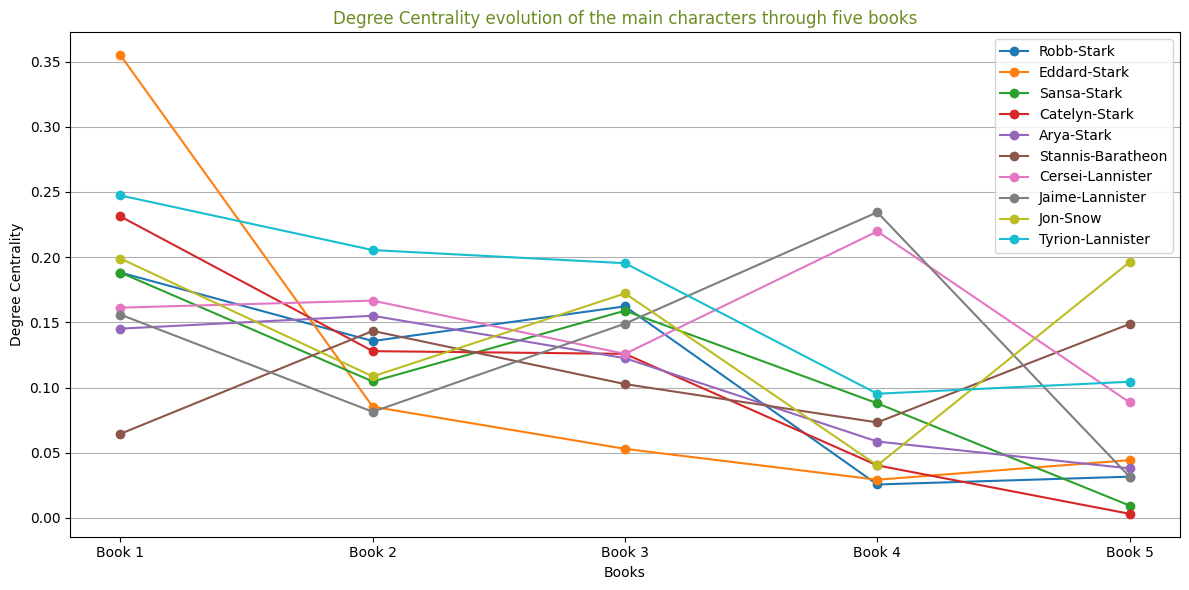
\includegraphics[width=0.8\textwidth]{deg-cent-evolution.png}
\caption{Degree Centrality evolution of the main characters through five books.}
\label{fig:deg_cent_evolution}
\end{figure}

\subsection*{Cliques}
We identified all cliques in each book's network. The largest cliques occur in the earlier books, where the narrative brings many main characters together. For example, in Book 1 one of the largest cliques included characters corresponding to the gathering of major figures at the King's Landing. We also found family-based cliques. Notably, the Stark family form a clique in Book 1. In later books, cliques tend to be smaller as the story splits geographically. This shows the data correctly captures close groups – whenever a set of characters all interact heavily, it appears as a clique, often aligning with narrative events like councils, feasts or family meetings. 
We focused on the largest cliques (of size greather than 3) and meaningful ones (like family cliques), since a great many trivial small cliques (triangles) exist. What cliques reveal is the community structure at its most strict definition: they highlight factions or scenes where everyone knows everyone else. 

A clique requires every possible edge to be present, which is a strong condition. Thus, many cohesive groups in the story won't appear as a full clique. We mitigated this by also examining k-cores and other measures for group cohesion. Nonetheless, clique analysis confirmed that the network representation picks up known close-knit groups, lending trustworthiness to the data extraction.

\subsection*{K-cores}

We performed a core decomposition to find k-cores. In each book, we found a clear highest-order core. In Book 1 and Book 2, the highest core was of order 11: for example, in Book 2 this 11-core contained ~12 characters centered on King Joffrey's court (essentially the Lannister family, the Kingsguard, and key council members in King's Landing). It reflects how tightly the royal court characters interlink. By Book 3, the maximum core was slightly lower (a 10-core with ~11 nodes), and it drops further in Book 4 and 5 (e.g. only a 7-core in Book 4). This trend quantifies the narrative's structural change: Book 1–2 have a very interconnected core cast (many characters all interacting in one place), whereas later books fragment the cast, so you cannot find as large a group all mutually connected. 

We found that the composition of the high-order cores aligns with major story factions.

K-cores give a layered view of network density. The highest k-core in each book essentially isolates the most central group of characters. We observed that these tend to be centered on political power hubs (court, major families). As k decreases, cores grow larger, bringing in progressively less-connected characters. It shows that even though hundreds of characters exist, the books have a relatively small inner-core driving interactions (often <20 characters).

One limitation is that k-core analysis ignores edge weights and treats all connections equally. Also, k-cores don't necessarily correspond exactly to narrative concepts of importance, they strictly capture connectivity. 

In general, K-core analysis supported that our network data is story-consistent: e.g. the cores we found contained coherent sets of characters, reinforcing that interactions were correctly identified.


\subsection*{K-components}

We analyzed k-components, which relate to the network's structural cohesion.

The story networks exhibited many small 2-components, but no giant 2-component containing all main characters. This indicates that the network has articulation points – characters whose removal would break apart the graph. 
We saw that most higher k-components were tiny groups of characters who form a fully interconnected cluster. 

For example, Arya Stark in Book 4 forms a 2-component with two of her Braavos contacts ("Waif" and the Kindly Man): Arya interacts with each of them and they interact (as teacher and fellow acolyte), making a triangle. One significant 2-component in Book 5 was Bran Stark's cohort beyond the Wall, forming a biconnected group; they are all in the same storyline, and they have multiple paths of interaction. 

The presence of such 2-components indicates pockets of the narrative that are very cohesive. 
 
The lack of a large 2-component including all major characters means the narrative has key "single points of failure". Indeed, if you "remove" certain central characters (for example, Tyrion Lannister in the early books), many others would lose their only connection and the network would fall into components. In fact, our analysis showed that the main giant component of each book is held together in part by a few critical connectors (which ties in with our betweenness findings). The small higher-order components we found (triads, small cliques) correspond to tightly-knit subgroups – typically members of the same family or people jointly involved in a particular subplot.

Our k-component analysis simply confirmed that, beyond the obvious cliques, the network contains no larger redundant sub-structures. Overall, the story graph is essentially tree-like: many branches extend from just a few trunk nodes. In practice, focusing on 2-components was enough, as we found no non-trivial 3-components.


\subsection*{Local Clustering Coefficient}
For each character, we calculated their local clustering coefficient.

We observed a wide range of LCC values, strongly correlated on a character's role. Major bridging characters had low clustering, whereas characters embedded in a single group had high clustering. 

In general, we found that characters who only appear within one close setting (e.g., members of the same household) often had very high clustering coefficients. In contrast, characters who serve as go-betweens connecting different groups had low LCC because those sets of neighbors don't interact with each other. 

We also looked at the average clustering: Book 1's average clustering coefficient was relatively higher than later books. This is intuitive since Book 1's main characters largely interact in one location (yielding interconnected neighbor sets). In later books, many characters have neighbors spread across disparate locales who never meet each other, lowering clustering. 

One  consideration is that, our co-occurrence network might count characters as "neighbors" if they are merely mentioned in the same chapter, even if they don't form a meaningful social tie.

\subsection*{Structural Equivalence} 
We examined how similar characters are in terms of whom they interact with. To compute this, we used metrics like the Jaccard coefficient, Pearson correlation, and Hamming distance. 

We found that perfect structural equivalence was rare. However, in Book 2, a trio of historical Targaryen princes (Aegon V, Daeron II, and Maekar I) are mentioned exclusively together in one anecdote; all three have the same neighbors, so any pair of them is structurally equivalent. 
The analysis didn't show any pair of major independent characters being extremely similar – which makes sense, since each protagonist has a unique journey. 

One caveat is that our similarity analysis rests on co-occurrence data, which can blur narrative roles. Two characters may appear in every scene together simply because they travel side by side, not because they serve the same plot function. Pearson correlation is also sensitive to differences in degree, so we used it mainly to validate what Jaccard revealed or to catch cases Jaccard missed.

We found that the top-ranked similarities were straightforward to interpret—mostly obvious co-travelers.

\subsection*{Jaccard Coefficient}

To measure how much two characters’ social circles overlap, we computed the
Jaccard coefficient for every pair of nodes.

The very few pairs that reach the maximum value of 1.0 are almost always
walk-on figures who appear together in a single scene or locale—for example,
\textit{Robert Arryn–Trystane Martell}, both merely mentioned in one small
council meeting in Book 2.  Because these cameo characters are seen only in the
company of the same handful of protagonists, they inherit identical
neighbourhoods and are effectively interchangeable background.

Conversely, pairs with a coefficient of 0.0—such as \textit{Addam Marbrand}
versus almost any peripheral Night’s Watch ranger—belong to storylines that
never intersect.  The large volume of zero-overlap pairs quantifies the
saga’s strong modularity: until later books, characters rooted in King’s
Landing politics have no common neighbours with those beyond the Wall or in
Essos.

Taken together, the distribution of Jaccard values reveals two key features
of the network.  First, extremely high scores cluster on peripheral nodes,
confirming that cameo characters are weakly embedded and gain their few links
solely from co-occurring with a single protagonist.  Second, the abundance of
zero scores maps the sharp boundaries between parallel narrative communities.

\subsection*{Pearson Correlation}

In our network the rare pairs that reach \(+1\) are almost always
walk-on figures who surface only alongside the same major characters.  
They serve as interchangeable background and never forge ties of their own.

At the other extreme, strongly negative—or near-zero—correlations arise
between protagonists such as Tyrion, Jon, Daenerys and Catelyn.
These leading characters act in storylines that are geographically and
socially isolated, each assembling a distinct entourage.

Thus, Pearson correlation does not underlie any important information with respect to the Jaccard Coefficient.

\subsection*{Hamming Distance}

Computing the Hamming Distance, we see that the biggest distances are almost always between main characters who live in separate story lines.
In Book 1 the pair "Eddard – Daenerys" has a huge distance.
Later books show the same pattern: Tyrion vs Jon, or Daenerys vs Stannis, get the top scores because each one moves with a unique group of allies and enemies.

On the opposite side, walk-on characters that appear together in the same single scene get a distance of zero.


So, the Hamming Distance confirms what we have found previously.

 
\subsection*{Regular Equivalence}

Our regular-equivalence analysis shows that each novel in A Song of Ice and Fire re-deploys a small set of structural templates—kings and queens, counsellors, heirs, and pretenders—even as the action shifts across continents.

 \begin{itemize}
     \item Book 1. The strongest equivalence links Eddard Stark and Robert Baratheon. Cersei Lannister scores next, her place in the royal triangle making her structurally close to both Eddard and Robert.
     \item Book 2. Tyrion and Joffrey emerge as the most equivalent pair: Tyrion rules as Acting Hand while Joffrey wears the crown, so they interact with virtually the same courtiers and guards.
     \item Book 4. Leadership is recast as a triad of Cersei, Tommen, and Margaery. The child-king and the two rival queens are tightly coupled to one another and to the shared Lannister–Tyrell power web.
     \item Book 5. The same royal pattern is transplanted to Meereen. At the centre stands Daenerys, whose closest equivalents are Hizdahr and Barristan. Quentyn, Daario.
 \end{itemize}

These patterns show that, even when the plot moves across continents, the social graph keeps re-using a limited set of structural templates—kings and queens, counsellors, heirs, pretenders-and regular equivalence is able to detect those templates automatically.

\subsection*{Homophily – Assortative Mixing}

Homophily is measured through the \emph{degree assortativity coefficient}, the Pearson correlation between the degrees of the two nodes at every edge.  
Across the five novels the coefficients are
\[
-0.166,\;-0.125,\;-0.133,\;-0.137,\;-0.185,
\]
and the aggregate network yields \(-0.133\).

\begin{itemize}
  \item \textbf{Disassortative structure.}  
        All coefficients are negative, so high-degree “hub” characters tend to connect with low-degree “peripheral” ones rather than with each other.  
        Each protagonist forms a local star: a central figure surrounded by minor characters who seldom interact among themselves—faithful to the vast, hierarchical world of Westeros.

  \item \textbf{Evolution across books.}
        \begin{itemize}
          \item \textbf{Book~2 (\(-0.125\)).}  
                The weakest disassortativity. Action is still clustered in King’s Landing, many characters share similar numbers of contacts, and the graph is less star-shaped.

          \item \textbf{Book~5 (\(-0.185\)).}  
                The strongest disassortativity. The narrative has splintered into distant theatres—Jon at the Wall, Tyrion on the run, Daenerys in Meereen, Stannis in the North.  
                Each lead gathers a new entourage of local extras, widening the degree gap between hub and neighbour.
        \end{itemize}
\end{itemize}

\medskip
In short, the increasingly negative assortativity quantifies the saga’s hierarchical social fabric: a handful of hubs mediate most interactions, and that hierarchy grows sharper as the plot spreads across continents.
\subsection*{Small-World Effect} 

All our character networks satisfy the classical "small-world'' condition.
For every book we computed the two standard indicators, 
$\sigma$ and $\omega$.
A graph is considered small-world when $\sigma>1$ or, equivalently, when $\omega$ is close to zero.
Book 1 already meets the requirement with $\sigma=1.64$ and $\omega=-0.07$, and the effect grows stronger through the series: $\sigma$ rises from $2.21$ in Book 2 to $2.81$ in Book 5, while $\omega$ stays in the narrow band $[-0.19,-0.07]$.
The aggregated five-book graph shows the same pattern, $\sigma=2.31$ and $\omega=-0.07$.

In practice this means that the story world is highly clustered families, 
courts and war camps produce many local triangles but, at the same time, 
any two characters are separated by only a few steps. 
Bridging figures such as Varys, Littlefinger, 
Tyrion or, later, Jon Snow and Daenerys act as 
shortcuts that link distant communities, keeping the average path length almost as low 
as in a random graph.  The monotonic increase of $\sigma$ from Book 1 to Book 5 reflects
 the geographic expansion of the plot: clustering grows because each new region adds its
  own dense sub-cast, yet the presence of travelling protagonists and frequent cross-mentions
   prevents the network from fragmenting, so the overall structure remains a textbook small world.


\subsection*{Degree Centrality} 
The log–log plots of degree centrality show a long tail: many characters have just one or two links, while a few "stars" (for example Tyrion, Daenerys or Eddard in their own books) collect a lot of connections.
We tried to fit the tail with a power law and obtained an exponent $\alpha$ that is not between 2 and 3, so the decay is steeper than in a classical scale-free network. In other words, our story graph has hubs. Because of this, random failure is dangerous: if we remove nodes without thinking, the chance to hit one of the big hubs is high and the graph can break apart quickly. From a narrative point of view it makes sense because most minor characters orbit around a small set of protagonists, so losing one key figure would disconnect many sub-plots at once.
\subsection*{Eigenvector Centrality}
Eigenvector centrality tells us who is important because they are linked to other important people.
In every single book the blue histogram on the left part of the figure is extremely skewed: most characters sit in the first bar, with a value smaller than $1$, while just a handful reach two, ten or even one hundred.  The cumulative curve on the right climbs slowly at the beginning and then rises very fast when it meets the first "elite" nodes; this shape is almost the same for Book 1, Book 2 and Book 3, gets a bit steeper in Book 4 and becomes even steeper in Book 5.  When we merge all books together the tail stretches over two full orders of magnitude, confirming that the saga always builds its plot around a micro-group of "star" characters whose prestige radiates through the whole network.

The pattern is intuitive: a king like Robert, a queen like Cersei or a leader like Daenerys does not only have many contacts, they are also directly connected to other high-status figures, so their eigenvector score explodes.  Minor knights, servants and one-chapter guests, instead, talk mainly to people as marginal as themselves and therefore keep a tiny value.  Because of this pyramidal structure the distribution cannot be fitted by a nice power law with an exponent between $2$ and $3$, so the network is not scale-free in the strict mathematical sense.  Nevertheless the evidence of a long heavy tail, together with the log–log straight segments that appear in the cumulative plots, tells us that power-law mechanisms are still present: the rich get richer, and the narrative keeps pushing attention towards the same protagonists while it introduces armies of low-impact side characters who quickly vanish from the story.

\subsection*{Closeness Centrality}
Closeness looks at distance: a character has high closeness if,
on average, she can reach every other node through only a few narrative "hops".


The histograms are bell shaped instead of heavy-tailed: most characters share a similar, medium closeness, while only a handful sit markedly closer to everyone else.  Those peaks correspond to the obvious hubs of the story, Eddard in \emph{Book1}, Tyrion in \emph{Book2-3}, Cersei in \emph{Book4}, and Daenerys plus Jon in \emph{Book5}.
From \emph{Book1} to \emph{Book5} the centre of the distribution drifts a little to the right, meaning that the typical distance among nodes becomes shorter: even if the cast grows, the narrative keeps adding shortcuts (for instance the war councils in the North and the royal courts in Meereen) that glue the network together.
When we put all books in a single graph the curve stretches further, 
yet the cumulative function on the right panel still reaches $F(x)\approx1$ 
very quickly; this tells us that the saga preserves a strong "small-village" feeling: 
information and conflict can spread almost everywhere in  few moves.

\subsection*{Betweenness Centrality}
The distribution of betweenness centrality highlights the narrative function of broker characters throughout the saga. In the first book the log–log histogram shows a very tall bar at values close to zero followed by a steep single–tailed decay that ends around ten. Most nodes therefore mediate no flow at all, while a handful act as genuine conduits; in story terms figures such as Tyrion, Cersei, Varys, and Littlefinger connect otherwise distant plots like Winterfell, the Wall, and the Dothraki sea.

In the second book the tail stretches slightly and additional bars appear between five and ten. The War of the Five Kings multiplies fronts and forces new intermediaries, for example Brienne or Davos, to occupy geodesic paths that had not existed before. The network becomes somewhat more integrated yet remains strongly hierarchical.

The third book displays the fattest tail of the series, indicating a larger number of bottlenecks. Many story lines converge in ensemble events such as the Red Wedding, and secondary characters linked to the Freys or the Boltons suddenly gain brokerage power before the plot fragments again.

In the fourth book the tail contracts: the narrative disperses across Dorne, Braavos, and the Iron Islands, so only a few actors centralise the traffic of information. Under these conditions betweenness is concentrated in a very small set of couriers or envoys who keep minimal ties among nearly independent arcs.

The fifth book widens the tail once more as new intersections arise among Jon, Stannis, and the diplomats of Meereen. Despite the geographic distance, characters like Jon, Tyrion, and Barristan reconnect clusters that would otherwise remain isolated, restoring some structural cohesion to the network.

When all books are merged the distribution takes the typical power-law form: an enormous mass of characters with negligible betweenness and a tiny elite that is always crucial. This confirms that the saga is scale–free: the bulk of the story is sustained by a few recurring brokers, while the majority stays peripheral.

Compared with eigenvector and closeness centrality, betweenness is the most unequal measure: more than seventy per cent of the nodes fall into the first histogram bin, whereas fewer than five per cent exceed double-digit values. Temporal evolution also reveals abrupt jumps: the death or exile of a key broker causes an immediate collapse of the index, while a successor records a sharp rise.

\subsection*{Local Clustering Coefficient}
The scatterplots that compare the average local clustering coefficient 
with degree centrality show a clear increase in every single book and in the combined network.

Characters with many interactions also belong to tightly knit neighbourhoods whose members
 are highly connected to each other, so the coefficient quickly rises toward one for medium
 to high degrees and then levels off. In contrast, characters on the edge of the story 
 have only a few links and much lower clustering, which means they appear in sparse or 
 short-lived contexts. This result matches the way the plot is organised. 
 
 The narrative moves across several separate locations such as Winterfell, King's Landing, 
 the Wall, and Essos, each with a fairly stable group of characters who mainly talk among 
 themselves.
 
 Within each location the social network is almost a clique, 
 so once a character becomes central there, the chance that any 
 two of their contacts have also interacted is close to certain. 
 This explains the flat top of the curves.
   The different steepness at the beginning of the curves reflects the shifting narrative focus.
   Books that emphasise court politics, especially Books 2 and 3, 
   have steeper slopes because the royal court is an exceptionally 
   dense conversational hub, while Book 4, which spreads attention over more places, 
   has a gentler rise. 
   
   Overall, the plots show that being a popular character is not only a personal trait but also a feature that emerges inside cohesive local communities whose members often appear together and exchange dialogue.

\subsection*{Density}
Network density is the fraction of all possible character pairs that actually interact. In Book 1 the density is 0.039 as the narrative stays mostly around the Stark family. Adding each new volume makes the network sparser, and when the five books are combined the density drops under one percent, because the roster of characters grows faster than the number of interactions.

\subsection*{Connectedness}
The connectedness index is equal to one for every book and for the combined network, indicating a graph where every node can be linked to every other through some path. 

\subsection*{Compactness}
None of the graphs for the five books shows high compactness, with values ranging from 0.193 to 0.150 and the full five-book network sitting at 0.160. That outcome fits the narrative structure as the story spreads across distant regions and many characters are separated by several intermediaries. 

\subsection*{Transitivity}
Transitivity tells us what share of all possible triangles of characters in the network are really present. The measure falls from 0.33 in Book 1 to 0.20 in Book 5, and when all five books are merged the score settles near 0.21. The steady decline confirms the growing geographic spread of the story through the books. 


\subsection*{Centralisation and Core-periphery Indices}
Centralisation tells us whether a few characters dominate the web of relations. In Book 1 degree centralisation is about 0.32, clearly higher than in the other volumes. Betweenness centralisation rises steadily from 48 in Book 1 to more than 140 in Book 5. This growth shows that the later books give more routing power to a small elite that sits on the critical bridges between story lines.

Core periphery analysis confirms the picture. 
When we split the graph by degree Book 1 produces a compact core of nodes surrounded by a looser rim, and the minimum rho value indicates that connections inside the periphery are rare. The optimal core grows with the cast, but the periphery always remains at least as large, meaning that most characters still live on the margins of the social space. 
K-core decomposition paints an even sharper contrast. 
In Book 1 the eleven-core includes only twenty three very resilient nodes; by Book 5 the threshold drops to six before we can collect a comparable dense nucleus, yet even then only seventeen names satisfy the condition and the remaining three hundred form the periphery. Taken together these indices show that the saga begins with a strongly centralised court and then spreads out geographically and socially, but a tiny set of pivotal figures continues to hold the network together and to channel the flow of information across its many regions.
  
\section{Conclusion}
\label{conclusion}

This project was set out to map and analyze the social network of characets in A song of Ice and Fire series, and our findings show that network analysis can indeed illuminate the story's Complex character dynamics.

By constructing a co-occurrence network for the five books, we identified key characters and examined how their roles change over time.

The various centrality measures consistently pointed to the most influential figures in the narrative.  At the same time, the metrics revealed some interesting insights, like the fact that Stannis Baratheon had an unexpectedly high betweenness centrality in the overall network.

This suggests that, despite not  having the most connections, Stannis serves as a crucial bridge between different storylines.

Similarly, secondary characters like Varys and Petrys Baelish stood out for linking otherwise separate groups.



Beyond individual characters, our analysis of the network’s structure uncovered patterns that align closely with the known factions and communities in the series. 
Clique detection and k-core decomposition showed that many tightly knit groups of characters in the network correspond to formal groups in the story,
 often members of the same house, location, or alliance. 
 For instance, one of the largest cliques in Book 1 was composed of Eddard Stark, his family, and close associates at King Robert’s court, 
 which reflects how these characters all interact in the same set of scenes. 
 In later books, the highest-order k-cores isolated clusters like the King’s Landing court or the Night’s Watch enclave, 
 mirroring the way the narrative splits into concurrent storylines. 

 These structural findings give us confidence that the network representation captures real story dynamics. 
 Global metrics further describe the shape of this fictional social world. 
 We found the network to be disassortative, meaning that highly connected hub characters tend to interact with many minor characters rather than with each other. 
 This produces a star-like hierarchy: each major character (a “hub” like Tyrion, Jon, or Daenerys) is surrounded by a circle of lesser-known characters, 
 much as in the books most secondary characters chiefly revolve around a main figure. 

 We also saw a clear small-world effect in Westeros: characters form locally clustered groups 
 (families, courts, traveling parties), yet a handful of bridge characters connect these groups so that any two characters are only a few steps apart. 
 This combination of very tight communities and short paths between characters reflects Martin’s storytelling, 
 where the world is sprawling but key figures link distant regions and plots. 
 
 Overall, the strong correspondence between our quantitative results and the novel’s narrative structure suggests that 
 our network-based approach captured meaningful aspects of character importance and relationships.

In summary, our work demonstrates the value of applying social network analysis to literature. We showed that numerical metrics can validate 
and enrich our understanding of a complex story: 
they confirmed known central characters, ranked characters by different notions of importance, 
traced how those roles evolve from book to book, and uncovered the presence of distinct communities and bridging roles. 
These insights complement traditional literary analysis by offering an evidence-based view of the story’s architecture. 

The significance of our study lies in this interdisciplinary approach, 
it connects computational methods with narrative analysis to shed light on how the story of Game of Thrones is structured. 

By quantifying character interactions, we not only reinforced what readers intuitively know about the saga’s heroes and factions, 
but also provided a new perspective on the social structure of the plot. 
This approach could be extended to other large narratives as well, suggesting that network science is a promising tool for exploring the social networks of fiction.
 

Future studies might build on this foundation by refining the network construction 
 (for example, distinguishing different types of interactions or weighting connections by their strength) 
 and by comparing our book-based network to other representations (such as the network in the television adaptation). 
 In the end, our project highlights how blending data-driven analysis with literary insight can deepen our understanding 
 of epic narratives like A Song of Ice and Fire.

\section{Critique}
Reflecting on our objectives, we believe that our work substantially solved the problem laid out in the introduction. 
The main goal was to find and measure character importance in a sprawling story with many characters and intersecting plotlines. 
In this respect, our analysis was quite successful: using social network metrics, 
we identified the principal characters in each book and in the series overall, 
and these largely matched the protagonists one would expect. We were able to quantify their importance from different angles
like connectivity, influence, brokering roles, and track how those measures changed as the story progressed. 



However, while we successfully answered many of our questions, some aspects can be explored further.
One reason is that character “importance” is a complex concept that cannot be fully captured by network centrality alone. 

Our analysis measured importance in terms of network structure. Essentially, how connected or structurally pivotal a character 
is in the co-occurrence graph. This did highlight narrative influence in many cases, but it might overlook characters who are important in more subtle ways. 
For instance, a character could be crucial to the plot without interacting with many others (perhaps acting behind the scenes or in a single storyline), 
and such a character would rank low in our network despite their narrative significance. In our findings, we saw that some characters known to be very 
important to the story’s outcome did not score top ranks in every metric: this suggests that our method captures one dimension of importance,
social connectivity, but not all dimensions (such as psychological or thematic importance). Additionally, the quality of our results depended 
on the dataset and assumptions we used. We relied on a co-occurrence network extracted from the text, which is an approximation of the true interaction network.
 
This approach sometimes connects characters who are merely mentioned together rather than directly interacting, and it treats all detected interactions as
  equal. These simplifications mean that our solution, while effective, has limitations. Therefore, we would say our project addressed the 
  research problem to a significant extent, it provided a strong structural analysis of character importance, 
  yet it leaves out some storytelling subtleties that a purely network-based method cannot capture.

There are several things we could have done differently to improve our answers to the research questions. 
First, we could gather more or different data to refine the network. 
Using the raw text of the novels with more advanced natural language processing might allow us to identify 
interactions more accurately. 
For example, distinguishing face-to-face dialogue from simple co-mentions, 
or noting whether an interaction is friendly or hostile. 
More detailed data could also include contextual information like chapter or location, 
which might help filter out incidental co-occurrences and focus on meaningful connections. 
Expanding the dataset beyond the books, for example by incorporating the TV show’s data or appendices that list character relationships,
could provide additional perspective and help verify the patterns we found. 

Second, we could use a different modeling approach for the network. Our current model is an unweighted, 
undirected graph built on co-occurrence within a fixed word window. 
A different approach might be to create a weighted network where edges have weights reflecting the strength or 
frequency of interactions between characters.
We could also consider a temporal or dynamic network model that evolves chapter by chapter or book by book, 
rather than just comparing static snapshots per book. This might capture the evolution of character importance more continuously.
Another modeling improvement would be to incorporate multiple types of relationships 
(for example, distinguishing family ties, alliances, or enmities as different layers in a multiplex network). 
Such richer models could better represent the story’s social complexity and possibly answer our questions more completely. 

Third, we might apply alternative metrics or analytical techniques to gain new insights. 
While we used a broad range of centrality measures and structural analyses, 
there are other angles we could explore. 
For instance, we could examine network resilience by simulating the removal of key characters to see how the structure breaks apart.
This would tell us more about which characters are truly irreplaceable in the network. 
We could also use community detection algorithms to automatically find groups of characters and compare those to known factions, 
rather than relying only on cliques and cores. 
Another idea would be to correlate our network-based rankings of character importance with external measures 
(such as how many chapters are told from a character’s perspective or fan popularity polls) 
to see if the network metrics align with other notions of importance. 

In retrospect, incorporating some of these additional methods might have provided a deeper or more nuanced answer to our questions.

In conclusion, our project made strong progress in solving the posed problem by using social network analysis to identify key characters and structural patterns in Game of Thrones. We achieved many of our goals by confirming major characters’ importance and uncovering the network’s features, but our solution is only partial in capturing the full richness of character importance. With more refined data, alternative modeling choices, and additional metrics, future work could address the remaining gaps. These improvements would allow for an even more comprehensive analysis, strengthening the bridge between quantitative network science and the qualitative art of storytelling.
\end{document}

